\documentclass[is,copyright,is]{isov2}
\usepackage{xeCJK}
\usepackage{booktabs}
\usepackage{amsmath}
\usepackage{caption}
\usepackage{graphicx}
\usepackage{indentfirst}
\usepackage{siunitx}
\usepackage{multirow}
\setlength{\parindent}{2em}
\setCJKmainfont[BoldFont={SourceHanSerifCN-Bold.otf}]{SourceHanSerifCN-Regular.otf}
%\setCJKmainfont{SimSun}
% preamble goes here
\renewcommand{\scopename}{范围}
\renewcommand{\forewordname}{前言}
\renewcommand{\defname}{术语和定义}
\renewcommand{\normrefsname}{规范参考}
\renewcommand{\introductionname}{序言}
\renewcommand{\figurename}{图}
\renewcommand{\listfigurename}{图目录}
\renewcommand{\listtablename}{表目录}
\renewcommand{\pagename}{页}
\renewcommand{\contentsname}{目录}
\renewcommand{\examplename}{例}
%\renewcommand{\listoftables}{表}
\renewcommand{\tablename}{表}
\renewcommand{\notename}{注}
\renewcommand{\annexname}{附录}
\usepackage{xcolor}
\usepackage{hyperref}
\hypersetup{
%	pdfborder= 0 0 0,
    colorlinks=true,
    linkcolor=blue,%
	pdfstartview={XYZ null null 1.00},
	pdfauthor = {汪卫},
	pdftitle = {全速自适应巡航系统},
}

\begin{document}

\standard{ISO 22179}
\yearofedition{2009}
\languageofedition{(E)}
\begin{foreword}
\fwdbp
\end{foreword}
\begin{introduction} % start Introduction
	 全速范围自适应巡航控制(FSRA)的主要系统功能是通过使用以下信息自适应地控制车辆速度:
	 \begin{enumerate}
	 	\item 离前车的车距;
	 	\item 本车(配有FRSA)的运动状态;
	 	\item 司机的操作指令(图\ref{fig:fsracontrolmode})。
	 \end{enumerate}
 根据所获得的信息,控制器(图\ref{fig:fsracontrolmode}中标识为“FSRA控制策略”)向执行器发送命令,执行其纵向控制策略,并将状态信息发送给司机。
\begin{figure}[htbp]
	\centering
	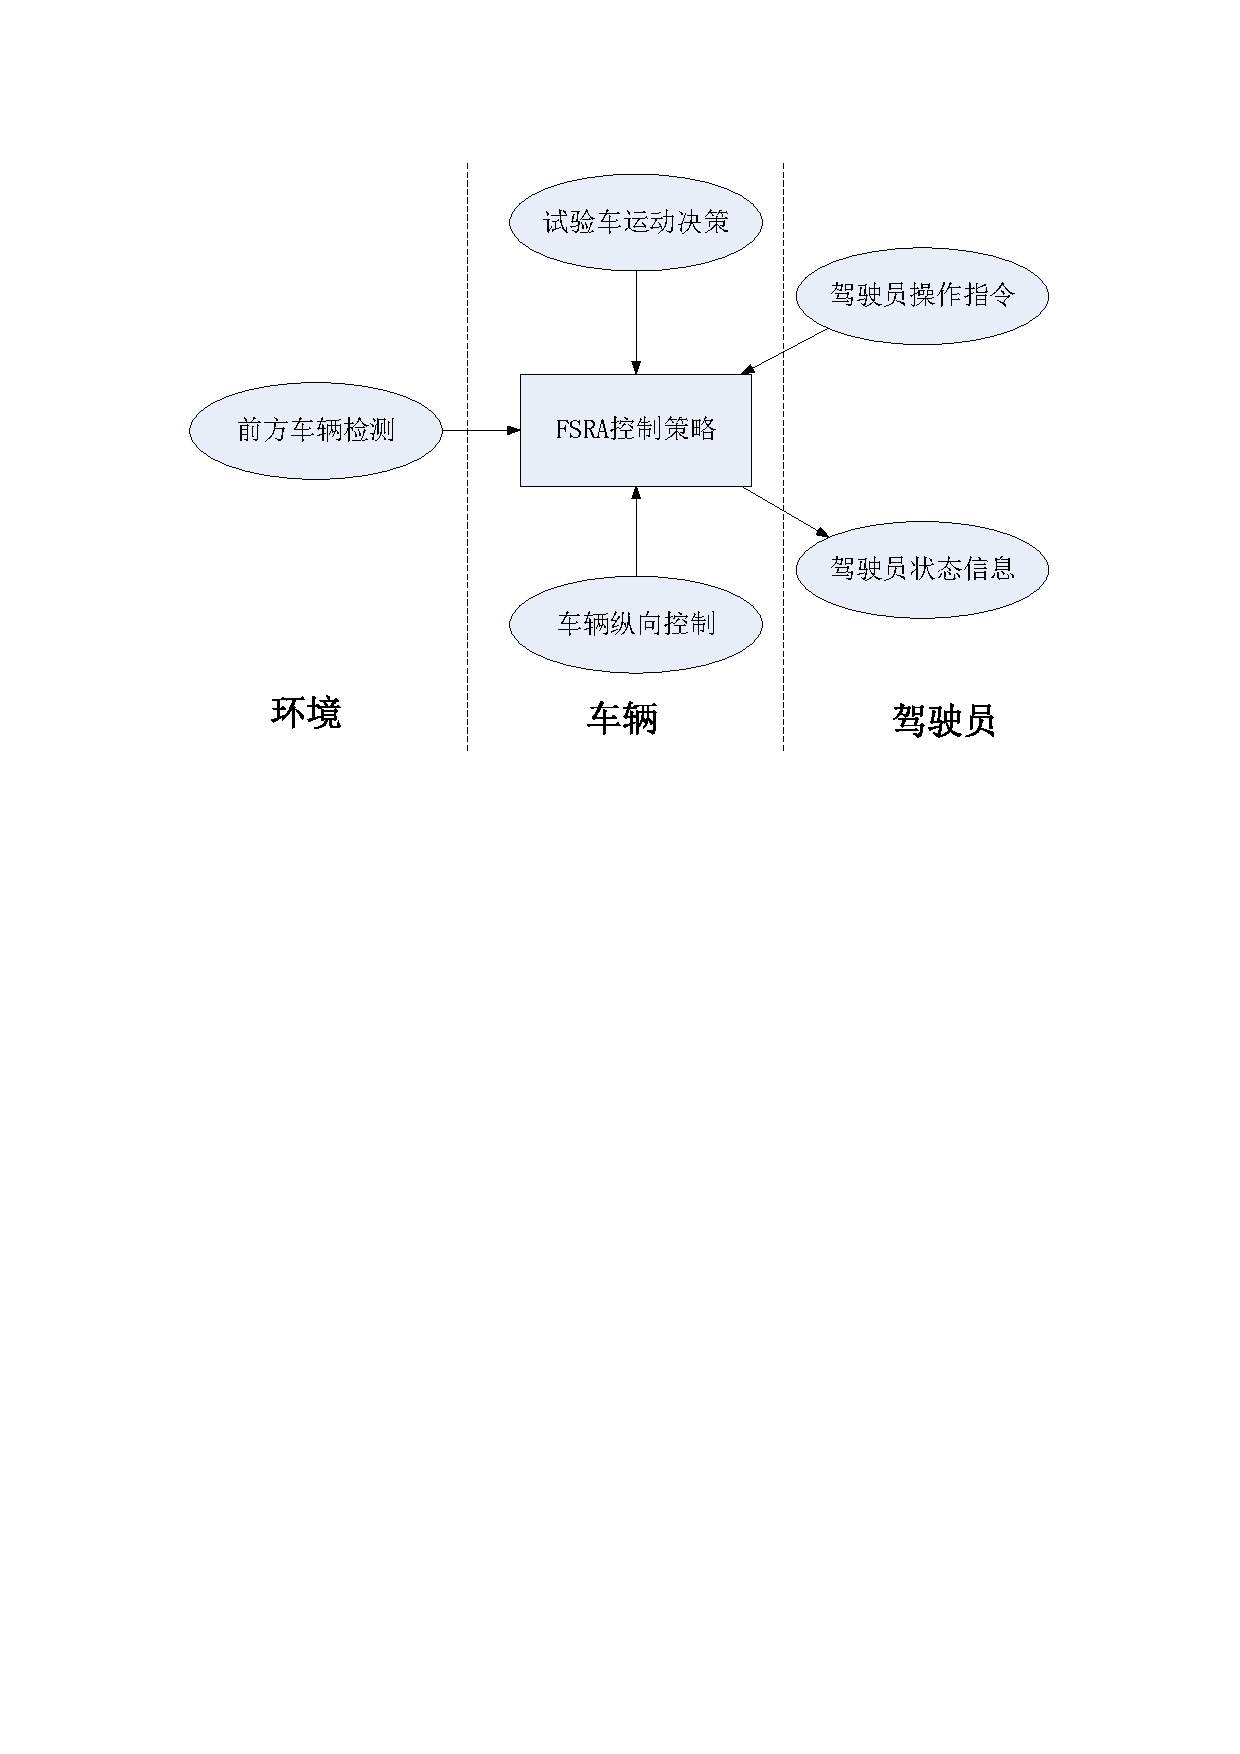
\includegraphics[width=0.7\linewidth]{figures/FSRAcontrolmode}
	\caption{FSRA功能的组成}
	\label{fig:fsracontrolmode}
\end{figure}
\end{introduction}
\title{\noindent 智能交通系统}%
{全速自适应巡航控制系统}%
{性能要求和试验规程}
FSRA的目标是纵向车辆控制的部分自动化,以减少驾驶员的工作量。

这个国际标准可以用作其他标准的系统级标准,这些标准将FSRA扩展到更详细的标准,例如, 用于特定检测和测距传感器概念或更高级别的功能。 诸如检测和测距传感器功能的具体要求等问题。本标准不考虑合作解决方案的性能或通信链接。
\scopeclause{本国际标准包含基本控制策略,最小功能要求,基本驾驶员交互元素,诊断和故障反应的最低要求以及全速范围自适应巡航控制(FSRA)系统的性能测试程序。 FSRA基本上旨在在高速公路(禁止非机动车辆和行人禁行的道路)在自由通行和拥挤的交通条件下行驶时对装备车辆进行纵向控制。 FSRA提供支持达到设计的系统最高速度以及停顿速度的范围。 系统将试图在有限的减速能力范围内停止已经跟踪的车辆,并且在驾驶员向系统输入要求从静止状态恢复之后将能够再次启动。 根据ISO 15622 自适应巡航控制(ACC),该系统不需要对静止或缓慢移动的物体作出反应。}
\normrefsclause % The Normative references clause
\begin{nreferences}
	\isref{ISO 2575}{Road vehicles — Symbols for controls, indicators and tell-tales}
\end{nreferences}
\defclause
本标准文档中的需要用得的专业术语含义:
\begin{definitions}
	\definition{主动制动控制}{\noindent 主动制动控制(active brake control ),由FSRA系统而不是驾驶员施加的制动控制动作。}
	\definition{自适应巡航控制}{\noindent 自适应巡航控制(Adaptive Cruise Control)是对常规巡航控制系统参见常规巡航控制(\ref{3.5})的改进,它可以通过控制本车发动机、传动系统或制动器实现与前车保持适当距离的目的。}
	\definition{制动}{\noindent 制动(brake),产生阻碍车辆运动或运动趋势的(制动力)的过程。}
	\begin{anexample}
		它可以是摩擦制动(由车辆上相对运动的两部分产生的摩擦力); 电动制动(由车辆上相对运动但不接触的两部分基于电磁作用产生的电磁力); 液力制动(由车辆上相对运动的两部分间的液体运动产生的阻尼力)时; 发动机制动(由发动机的制动作用产生的传递到⻋轮的制动力)。
	\end{anexample}
	\begin{note}
	采用的ECE-R 13-H标准定义,但就本国际标准而言,其中传动控制装置的制动不予考虑。
    \end{note}
 \definition{车间距}{\noindent 车间距(clearance),前车尾部与本车头部之间的距离。}
 \definition{常规巡航控制}{\noindent 常规巡航控制(conventional cruise control),按照驾驶员的设定控制车辆行驶速度的巡航系统。}\label{3.5}
 \definition{前车}{\noindent 前车(Forward Vehicle),与本车同向、同路,并在本车前方行驶的车辆。}
 \definition{自由流交通}{\noindent 自由流动的路况(free-flowing traffic)车流量大但比较流畅的交通,不包括频繁起步停车和紧急制动的情况。}
 \definition{车间时距}{\noindent 车间时距(time gap),$\tau$,本车驶过连续车辆的车间距所需的时间间隔。由试验车速$v$,以及距离前车距离$c$,计算所得:$\tau =c/v $。}
  \begin{anote}
 	见图~\ref{fig:timegap}。
 \end{anote}
\begin{figure}[htbp]
	\centering
	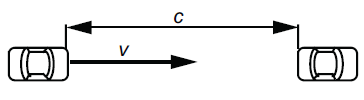
\includegraphics[width=0.6\linewidth]{figures/timegap}
	\caption{车间时距}
	\label{fig:timegap}
\end{figure}
 \definition{设定速度}{\noindent 设定速度(set speed),期望的行驶速度,由驾驶员或由FSRA系统以外的其他控制系统设定的期望行驶速度。}
 \begin{anote}
 车辆在FSRA系统控制下的最高期望速度。
  \end{anote}
 \definition{稳定状态}{\noindent 稳定状态(steady state),相关参数不随时间、距离变化的车辆状态。}

  \definition{本车}{\noindent subject vehicle 配有FSRA功能的车辆,即本标准讨论的车辆。}
  \definition{系统状态}{\noindent 系统的工作状态(
  	见图~\ref{fig:fsramode})。}
\begin{definitions}
    	 \definition{FSRA关闭状态}{\noindent FSRA关闭状态(FSRA off state),用于激活“FSRA激活状态”的直接访问被禁用的状态}
    	 \definition{FSRA待机状态}{\noindent FSRA待机状态(FSRA 待命状态),FSRA系统没有纵向控制的状态,并且系统准备好由驾驶员激活。}
    	 \definition{FSRA工作状态}{\noindent FSRA激活状态(FSRA active state),系统处在可以控制速度和或间距的状态。}
    	 \definition{FSRA保持状态}{\noindent FSRA保持状态(FSRA hold state),本车在静止的过程中,系统处于FSRA激活状态。}
    	 \definition{FSRA速度控制状态}{\noindent FSRA速度控制状态(FSRA speed control state),系统根据设定速度控制速度的状态。}
    	 \definition{FSRA跟随控制状态}{\noindent FSRA跟随控制状态(FSRA following control state),系统根据选定的车间时距控制到目标车辆的车距的状态。}
\end{definitions}
\definition{目标车}{\noindent target vehicle,本车跟随的车辆。}
\definition{慢速移动目标}{\noindent slow moving object,在本车前的以小于MAX[\SI{10}{m/s},10\%的主车速]移动目标。}
\definition{静止目标}{\noindent stationary object,本车前方的静止物体}
\definition{全速自适应巡航系统}{\noindent full speed range adaptive cruise control,自适应巡航控制系统的增强系统。可以通过控制发动机和(或)动力传动系以及制动器使车至静止状态,使本车以适当的距离跟随前方车辆。}
\end{definitions}
\clause{符号和缩写术语}
\begin{symbols}
	 \symboldef{$a_\text{lateral-max}$}{ 弯曲道路上的最大横向加速度}
	 \symboldef{$a_\text{stopping}$}{自动“停止”能力测试中的横向停止加速度}
	 \symboldef{CCT}{ 红外反射器测试目标系数}
	 \symboldef{RCS}{radar cross-section 雷达截面}
	 \symboldef{$c$}{车距}
	 \symboldef{$c_\text{min}$}{稳定状态下的最小车距}
	 \symboldef{$d_0$}{判断是否有必要探测目标车辆的临界距离}
     \symboldef{$d_1$}{判否有必要测量距离或相对速度的临界距离}
     \symboldef{$d_2$}{需果测量操作的距离}
     \symboldef{$d_\text{max}$}{直线道路上的最大探测距离}
     \symboldef{LIDAR}{激光雷达}
     \symboldef{R}{弯道半径}
     \symboldef{$R_\text{min}$}{弯道最小半径}
     \symboldef{$v_\text{circle}$}{弯道上,当给定最大横向加速度$a_\text{lateral-max}$时的最高车速}
     \symboldef{$v_\text{circle-start}$}{车辆进人半径为R的弯道时的初始速}
     \symboldef{$v_\text{set-max}$}{最大可选测试速度}
     \symboldef{$v_\text{set-min}$}{最小可选测试速度}
     \symboldef{$v_\text{stopping}$}{自动“停止”能力测试中的本车速度}
     \symboldef{$v_\text{vehicle-end}$}{测试结束时的车速}
      \symboldef{$v_\text{vehicle-start}$}{测试开始时的车速}
      \symboldef{$v_\text{vehicle-start}$}{测试的最高车速}
       \symboldef{$\tau$}{车间时距}
       \symboldef{$\tau_\text{max}$}{可供选择的最大车间时距}
       \symboldef{$\tau_\text{min}$}{可供选择的最小车间时距}
        \symboldef{$\tau_\text{min}$}{当给定车速$v$时,可供选择的最大车间时距}
\end{symbols}

\clause{分类}
本国际标准适用于表~\ref{tab:ACCperformancespec}中规定的具有不同弯道行驶适应能力的FSRA系统。
\begin{table}[htbp]
	\centering
	\caption{基于弯道行驶能力的FSRA系统分类}
	\begin{tabular}{|c|c|}
		\hline
		性能类型    &对弯道半径的适应能力(m) \\
		\hline
		I    & ACC(ISO15622)中保留,不适用FSRA  \\
		\hline
		II    & $\geq 500 $   \\
		\hline
		III    & $\geq 250 $   \\
		\hline
		IV    &  $\geq 125 m$   \\
		\hline
	\end{tabular}%
	\label{tab:ACCperformancespec}%
\end{table}%

\clause{要求}
\sclause{基本控制策略}
\begin{figure}[htbp]
	\centering
	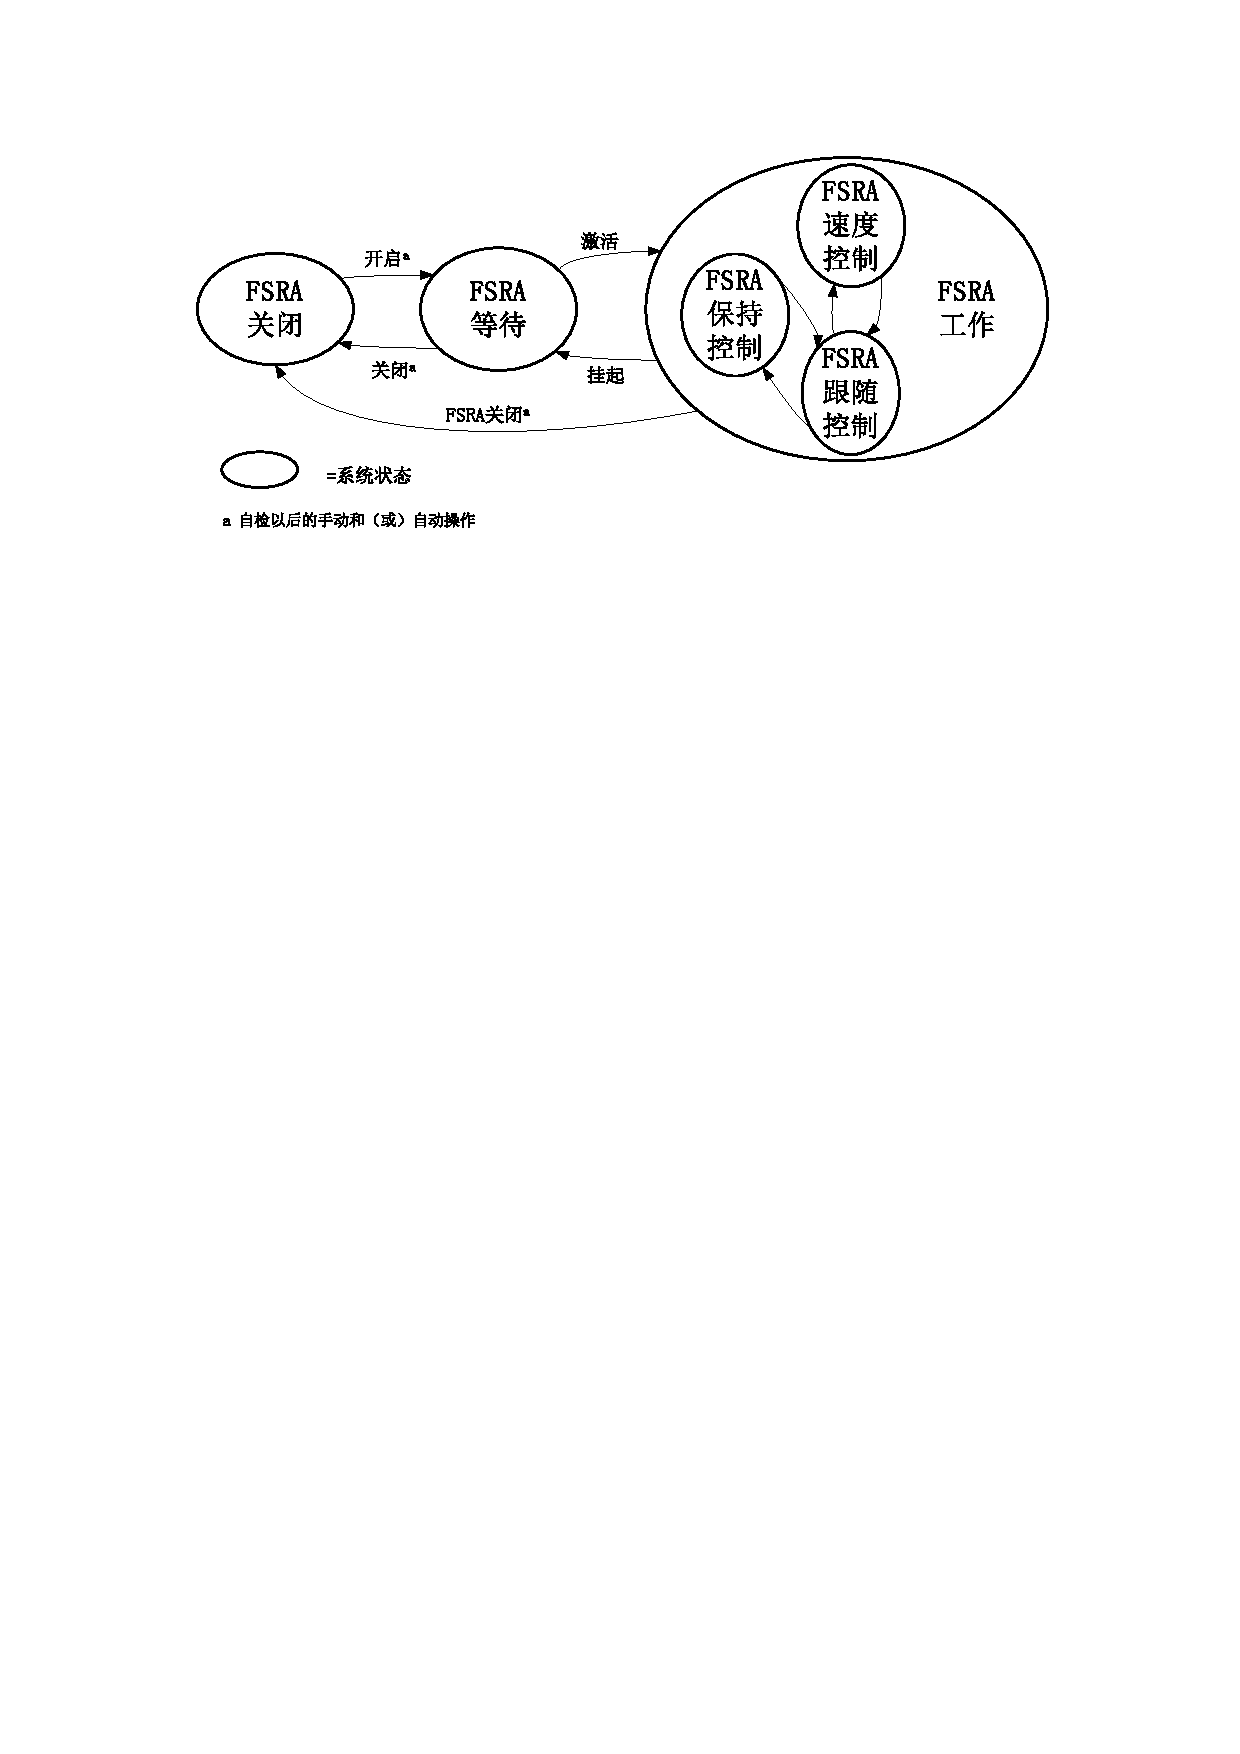
\includegraphics[width=0.7\linewidth]{figures/FSRAmode}
	\caption{FSRA状态及其切换}
	\label{fig:fsramode}
\end{figure}

\begin{anote}
	手动转换描述了一个用于启用/禁用FSRA功能的开关,自动关闭可以由故障反应强制触发。
\end{anote}

FSRA系统至少应提供以下控制策略和状态转换。以下构成FSRA系统的基本行为。

\begin{enumerate}
	\item 当FSRA处于激活状态时,本车通过对速度的自动控制来与前车保持一定的车间时距或预先的设定速度(以二者中速度低者为准)。这两种控制模式之间的转换可由FSRA系统自动完成。
	\item 稳态间隙可以由系统自行调节或由驾驶员调节。
	\item 如果本车的前方有多辆车,系统应自动选择要被跟随的车辆
	\item 主车停止后,系统状态应在三秒内,实现跟随状态到保持状态。
	\item 处于保持状态时,制动控制系统应能保持本车静止。
\end{enumerate}


\sclause{功能}
\ssclause{控制模式}
控制模式(车间时距控制和车速控制)之间的转换应自动进行。。
\ssclause{静止或慢速移动目标}

该系统将试图在有限的减速能力范围内停车在已追踪并停车的车辆的后面。 设计以响应固定或缓慢移动目标的FSRA系统是可选的。 如果给定的实施方案不打算响应固定或缓慢移动的目标,应至少通过车主手册中的声明通知驾驶员。
\ssclause{跟车能力}\label{6.2.4}
\begin{symbols}
	\symboldef{$\tau_\text{min}$}{稳定状态下的跟随控制模式对于所有车速$v$,有可供选择的最短车间时距,$\tau_\text{min}$应大于等于1s}
	\symboldef{$c_\text{stopping}$}{稳定状态下的跟随控制模式对于所有车速$v$,有可供选项的最短车距,最短车距至少2m}
\end{symbols}

在稳定状态下,最短车距应为$\max(c_\text{min},\tau_\text{min}\times v)$。在中间状态下车距可能会瞬时降到最短车距下。如果出现此种情况,系统应调整车距来实现目标车距。


对于车速超过$\SI{8}{m/s}$应提供至少一个时间间隔设定$\tau$,其范围为1.5 s至2.2s。

作为最低要求,本车从稳态跟车开始,系统应能减速跟停在减速度为$a_\text{stopping}$,减速度为$v_\text{stopp}$的后面(测试程序见7.3.2),其中:

$v_\text{stopping} = \SI{10}{m/s}$

$a_\text{stopping}=\SI{2.5}{m/s^2}$

\sssclause{}
FSRA应具备以下的检测距离、目标识别、弯道适应能力。
\sssclause{}
直线道路上测距(适用于II,III,IV型)

如果前车位于$d_1$至$d_\text{max}$的距离范围内,则FSRA系统需要测量本车与前车之间的距离(见图~\ref{fig:zonesofdetection})。在此距离范围内,前车应能检测到的水平区域不低于本车宽度。 

\[d_\text{max} = \tau_\text{max}(v_\text{set-max})\times v_\text{set-max}\]

如果前车位于$d_0$到$d_1$的距离范围内,FSRA系统需要探测前车的存在,而不需要测量本车和前车之间的距离或相对速度。
\[d_1 = \SI{4}{m}\]

如果前车的距离位于$d_0$范围内,则FSRA系统不需要检测车辆的存在。
\[d_0 =\SI{2}{m} \]
\begin{figure}[htbp]
	\centering
	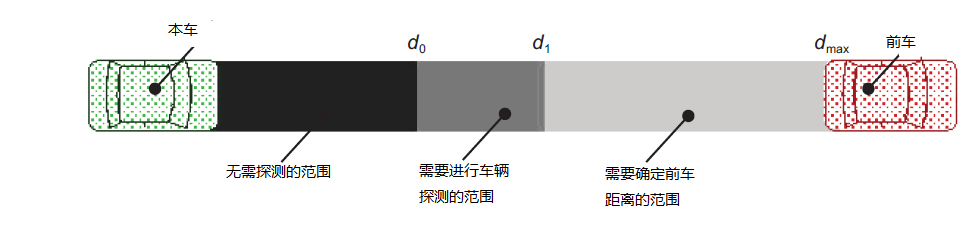
\includegraphics[width=0.7\linewidth]{figures/zonesofdetection}
	\caption{检测范围}
	\label{fig:zonesofdetection}
\end{figure}
\sssclause{目标识别能力}\label{sec:disc}

如果在直道上前方存在多辆车,或者在弯道上并且本车的FSRA系统属于II + III + IV型,则与本车处于同一车道的前车(见图~\ref{fig:targetdisciminnation})将被选作FSRA控制的目标车,检测方法见)。具体见7.5
\begin{figure}[htbp]
	\centering
	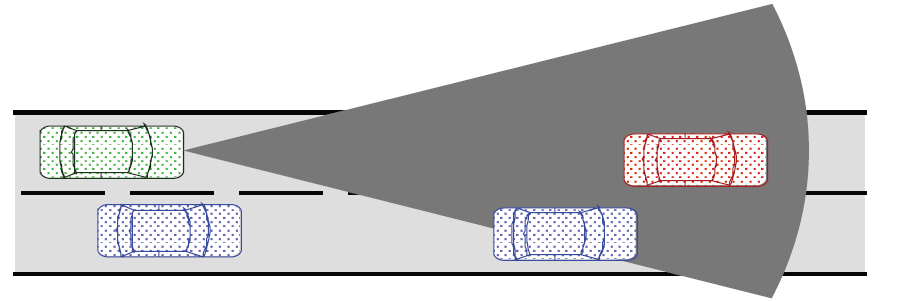
\includegraphics[width=0.7\linewidth]{figures/targetdisciminnation}
	\caption{目标识别}
	\label{fig:targetdisciminnation}
\end{figure}

\sssclause{弯道适应能力(性能等级II,III,IV)\label{sec:curetest}}

FSRA系统能够使车辆在直道和弯道上以车间时距$\tau_\text{max}(v_\text{circle})$稳定跟随前车行驶。因此,如果前车沿半径为$R_\text{min}$的弯道以恒速$v_\text{circle}$行驶,FSRA系统可使本车以稳定的车间时距$\tau_\text{max}(v_\text{circle})$跟随前车。不同类型的FSRA系统对弯道半径的适应能力不同:I型仅适应于直道(可认为半径为无穷大);II型可适应的弯道最小半径为$R_\text{min,II} = 500$m;III型可适应的弯道最小半径为=$R_\text{min,III} = 250$m; IV 型可适应的弯道最小半径为$R_\text{min,IV} = 125$m。

\[v_\text{circle} = \sqrt{a_\text{lateral-max}\times R_{min}}\]
其中:

$\tau_\text{max}(v)$ --- 当车辆以速度$v$行驶时的车间时距的最大稳定值;

$a_\text{lateral-max}$ --- 是曲线公路上的设计横向加速度,公路弯道上的最大设计横向加速度,其取值如下:

$ a_\text{lateral-max,II} = 2.0 \si{m/s^2}$

$ a_\text{lateral-max,III} = 2.3 \si{m/s^2}$

$ a_\text{lateral-max,IV} = 2.3 \si{m/s^2}$

$a_\text{lateral-max}$的值基于驾驶员的平均驾驶水平获得(95\%驾驶员),具体见图~\ref{fig:lateralacceleration}和参考文献\ref{ref:UN}。
\begin{figure}[htbp]
	\centering
	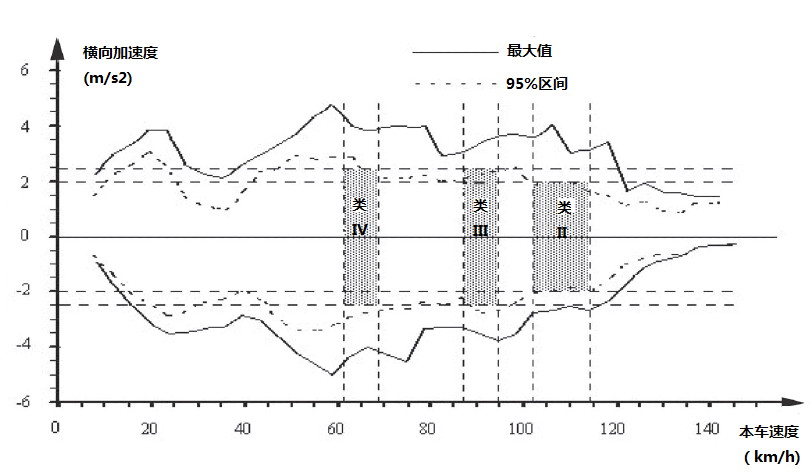
\includegraphics[width=0.6\linewidth]{figures/lateralacceleration}
	\caption{一般驾驶员的横向加速度}
	\label{fig:lateralacceleration}
\end{figure}

\ssclause{“go” 转换}
从保持到跟车控制或速度控制的转变需要驾驶员命令才能触发。
\sclause{基本的人机交互功能}

\ssclause{操作和系统反应}

\sssclause{}
FSRA系统应为驾驶员提供一种用来选择并设定期望车速的方法
\sssclause{}
FSRA处于跟随控制和速度控制状态时,如果驾驶员初始制动力命令高于FSRA初始制动力,驾驶员的制动应使FSRA功能失效。在FSRA保持状态,不强制要求驾驶员制动使FSRA系统失效[若制动,会使FSRA切换到待机状态,见图(~\ref{fig:fsramode})]。
\sssclause{}
即使在FSRA系统处于自动制动的情况下,FSRA系统不应明显地削弱车辆对驾驶员制动输人的瞬时响应能力 (见ECE-R 13-H)。

\sssclause{}
当驾驶员与FSRA系统均有发动机动力控制(节气门输人)请求时,以二者中的大者为准,这将使驾驶员对发动机动力控制的优先权始终髙于FSRA系统。

如果驾驶员的动力需求高于FSRA系统时,FSRA系统的自动制动力应立即释放。对驾驶员控制加速踏板不应有明显的响应延迟。
\sssclause{}
自动制动状态对车轮的抱死时间不应超过ABS的允许值。该项要求无论系统有无ABS系统均适用。
\sssclause{}
 FSRA系统的发动机动力控制作用引起的车轮打滑时间不应超过牵引力控制系统的允许值。 FSRA系统不干涉牵引力控制系统。
\sssclause{}
FSRA系统可适当调整车间时距以适应驾驶环境的变化(如恶劣天气),但被调整后的车间时距不应低于驾驶员的设定值。
\sssclause{}
如果FSRA系统允许驾驶员选择期望的车间时距,应采取以下几种方法之一:
\begin{enumerate}
	\item 如果FSRA系统关闭后仍存储着最近一次选定的车间时距值(见图~\ref{fig:fsramode}),则当系统被再次激活后,应将该车间时距值显示给驾驶员;
	\item 如果FSRA系统关闭后不存储最近选定过的车间时距值(见图~\ref{fig:fsramode}),则车间时距应被设定为默认值(大于或等于1.5 s)
\end{enumerate}
\sssclause{}
如果车辆同时配备有ACC系统和常规巡航控制系统,则二者之间不应自动切换。
\sssclause{}
可选地,系统可能在静止的状态下被驾驶员激活,即使即使有踩了制动板。
\ssclause{显示}
\begin{enumerate}
	\item 为驾驶员提供最基本的反馈信息,包括FSRA系统状态以及设定速度等,并且它们可以组合在一起显示输出,例如仅在FSRA工作时显示设定速度。
	\item  如果FSRA系统失效或出现故障,应及时提示驾驶员,提示符号应符合标准(见\ref{sec:symbol})。
	\item 如果车辆同时配备有ACC系统和常规巡航控制系统,则应向驾驶员提示当前处于工作状态的系统。
	\item 采用信息“探测到车辆”来表示FSRA系统已探测到前方有一车辆,可作为控制的参考目标。
\end{enumerate}

\ssclause{符号}\label{sec:symbol}
如果采用符号来标识FSRA系统的功能和故障状态,应符合ISO 2575的规定。
\sclause{操作限制}\label{6.4}
为了改善舒适性,对于低于$\SI{5}{m/s}$的车速,因目标车消失或系统自动失效,系统不应出现突然制动力。

最低的设定车速应$v_\text{set-min} \geq\SI{7}{m/s}$。

当车以 $\SI{20}{m/s}$行驶时,FSRA系统的平均减速度不应大于$\SI{3.5}{m/s^2}$ (以2s的长度按采样值求平均)。当车以低于 $\SI{5}{m/s}$行驶时,FSRA系统的平均减速度不应大于$\SI{5}{m/s^2}$。具体见图\ref{fig:dmax}
\begin{figure}[htbp]
	\centering
	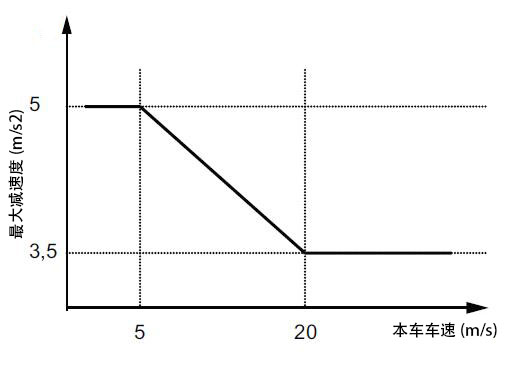
\includegraphics[width=0.7\linewidth]{figures/dmax}
	\caption{本车最大减速度}
	\label{fig:dmax}
\end{figure}

当车以 $\SI{20}{m/s}$行驶时,FSRA系统的平均减速度率不应大于$\SI{2.5}{m/s^3}$ (平均超过1s)。当车以低于 $\SI{5}{m/s}$行驶时,FSRA系统的平均减速度率不应大于$\SI{5}{m/s^3}$。具体见图\ref{fig:jerkmax}
\begin{figure}[htbp]
	\centering
	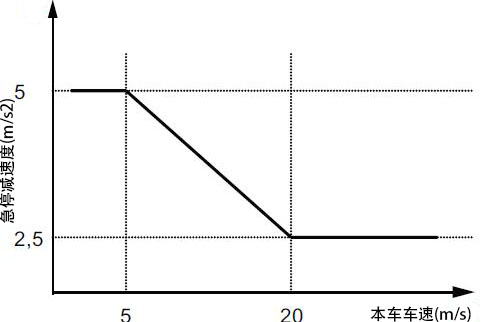
\includegraphics[width=0.7\linewidth]{figures/jerkmax}
	\caption{最大急停速度与加速度关系}
	\label{fig:jerkmax}
\end{figure}


当车以 $\SI{20}{m/s}$行驶时,FSRA系统的平均加速度率不应大于$\SI{2}{m/s^3}$ (平均超过1s)。当车以低于 $\SI{5}{m/s}$行驶时,FSRA系统的平均加速度率不应大于$\SI{4}{m/s^3}$,见图~\ref{fig:amax}。
\begin{figure}[htbp]
	\centering
	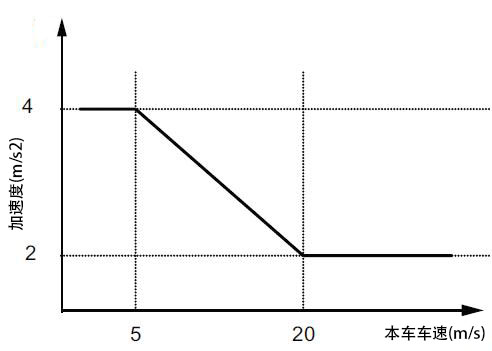
\includegraphics[width=0.7\linewidth]{figures/amax}
	\caption{最大加速度}
	\label{fig:amax}
\end{figure}

如果目标车接近$d_0$但是没有检测到时,系统应该初始化一种控制器策略,作用范围是从上次有效制动命令开始,直到本车停下来或系统检测到$d_1$范围内或驾驶员通过加速脚踏板取代系统。如果在$d_0$到$d_1$范围内检测到前车,同时检测距离不能确定,系统应禁止自动加速。
\sclause{制动灯激活控制}
如果FSRA系统工作过程中进行自动制动操作,则应点亮制动灯,当FSRA系统执行了其他减速操作时制动灯也可被点亮。制动灯点亮动作应该在FSRA系统开始制动操作后的350 ms以内完成。为防止制动灯忽亮忽暗,在FSRA结束制动之后可维持制动灯亮一个合理的时间。
\sclause{故障反应}
\begin{enumerate}
	\item 表2给出了子系统失效的情况下的FSRA系统所需的故障反应(见图\ref{fig:acccontrolmode})
	\item 表2列举的故障应立即提示驾驶员,提示信息应保持至系统关闭。
	\item FSRA系统重新开启之前应完成系统自检才能开启,自检过程可由点火开关或FSRA系统开关触发
\end{enumerate}
\begin{figure}[htbp]
	\centering
	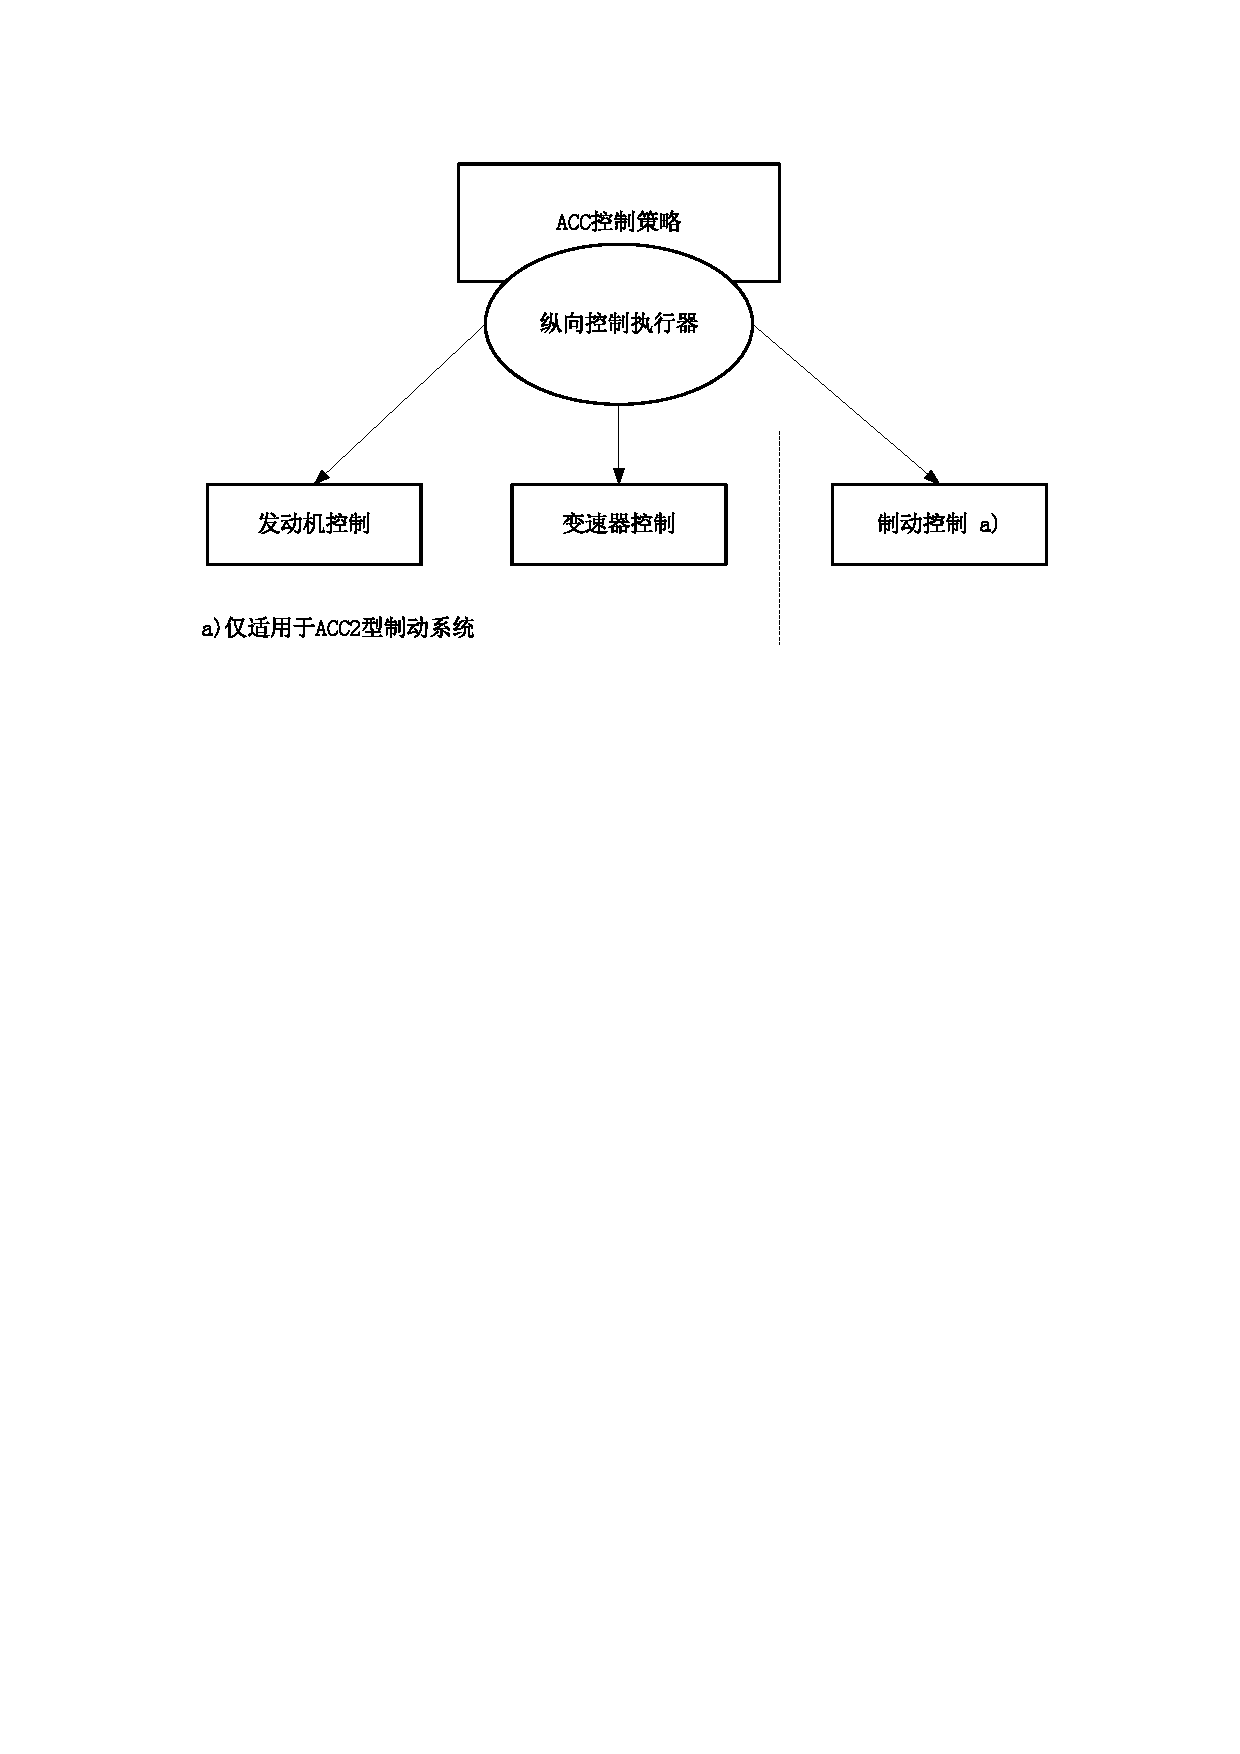
\includegraphics[width=0.7\linewidth]{../ACCnew/figures/ACCcontrolmode}
	\caption{纵向控制执行器}
	\label{fig:acccontrolmode}
\end{figure}

\begin{table}[htbp]
	\centering
	\caption{FSRA故障处理}
	\begin{tabular}{|p{10em}|c|c|}
		\hline
		\multirow{2}[4]{*}{故障子系统} & \multicolumn{2}{p{30em}|}{发生故障时FSRA系统的工作模式} \\
		\cline{2-3}    \multicolumn{1}{|c|}{} & \multicolumn{1}{p{15em}|}{制动控制模式} & \multicolumn{1}{p{15em}|}{发动机控制模式} \\
		\hline
		发动机   & \multicolumn{1}{p{15em}|}{应保持制动,至少为满足当前的制动操作需要} & \multicolumn{1}{p{15em}|}{放弃FSRA的发动机控制模式} \\
		\hline
		制动系统 & \multicolumn{1}{p{10em}|}{放弃FSRA控制模式} & \multicolumn{1}{p{10em}|}{放弃FSRA的发动机控制模式} \\
			\hline
		探测和距离传感器 & \multicolumn{1}{p{20em}|}{利用最近使用过的有效的制动指令启动一个控制策略。一旦驾驶员操纵制动踏板或加速踏板或FSRA开关,系统立即关闭} & \multicolumn{1}{p{15em}|}{放弃FSRA的发动机控制模式} \\
			\hline
		FSRA控制器 & \multicolumn{1}{p{20em}|}{放弃FSRA控制模式} & \multicolumn{1}{p{15em}|}{放弃FSRA控制模式} \\
		\hline
		\multicolumn{3}{|p{30em}|}{如果变速器出现故障,制动操作应能完成减速功能} \\
		\bottomrule
	\end{tabular}%
	\label{tab:acc2a}%
\end{table}%
\clause{性能评价测试方法}
\sclause{测试环境条件}
测试环境条件如下:
\begin{enumerate}
	\item 测试场地为平坦干燥的沥青或混凝土路面;
	\item 温度应在$\SI{-20}{\celsius}\sim \SI{40}{\celsius}$;
	\item 水平能见度应大于$\SI{1}{km}$
\end{enumerate}
\sclause{测试目标规范}\label{7.2}
\ssclause{采用激光雷达测试时:}
红外线的测试目标是由一个测试目标的红外线系数CTT和测试目标的横截面定义。测试目标A与B的最小反射横截面为$\SI{20}{cm^2}$;
\begin{itemize}
	\item 测试目标A属于漫反射体,其$\text{CCT} = \SI{2.0}{m^2/sr} \pm 10\% $(见附录A);
	\item 测试目标B属于漫反射体,$\text{CCT} = (1.0 \pm 0.1)\si{m^2/sr} $;
\end{itemize}
\ssclause{采用毫米波雷达测试时:}
测试目标由雷达信号的散射横截面(RCS)定义。

频率范围为$\SI{20}{G\hertz}\sim \SI{95}{G\hertz} $。
\begin{itemize}
	\item 测试目标A的RCS应为\SI{10}{m^2};
	\item 测试目标B的RCS应为\SI{3}{cm^2}。
\end{itemize}
对于明显不同的频率范围,RCS应重新确定和定义(见附录A)。

\sclause{自动“静止”能力测试}
\ssclause{测试目标车}
测试目标应具备~\ref{7.2}节所定义的测试目标A要求。测试目标应放置在车辆的后部。其余未被遮盖的表面按如下原则进行隐藏处理:使车辆尾部的雷达散射截面RCS不大于(移去测试目标A以后)或使其反射率不大于测试目标的20\%。
\ssclause{初始条件}
测试目标应以$v_\text{stopping}$的速度行驶。

测试目标车的宽度在1.4m到2.0m范围内。

本车以稳定状态模式跟随测试目标车。

全程测试过程中,最佳车距时距应为$\tau_\text{min}$。

本车与目标车纵向中心线间的横向偏差小于0.5m(见图\ref{fig:stopcap})
\begin{figure}[htbp]
	\centering
	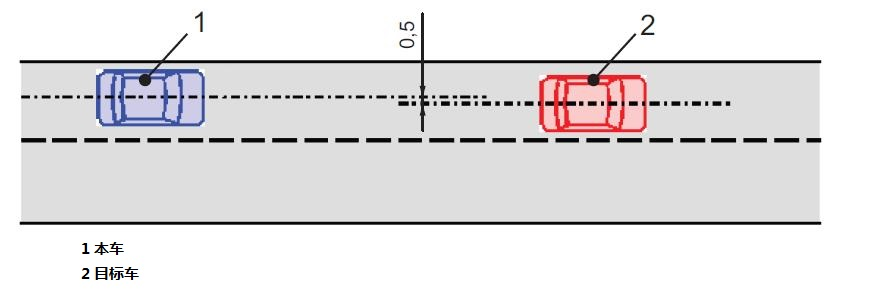
\includegraphics[width=0.7\linewidth]{figures/stopcap}
	\caption{自动禁止能力测试(初始条件)}
	\label{fig:stopcap}
\end{figure}

\ssclause{测试程序}
测试目标车减速度应为$a_\text{stopping} - 0.5 $\si{m/s^2}。

当系统制动下本车静止停止在前车后面时,测试目标才能视为成果。

\sclause{探测距离测试\label{sec:detectionspec}}
探测距离$d_0,d_1,d_2,d_\text{max}$的测试程序:

车辆参考平面为一矩形,宽度与本车宽度相当,高0.9 m,离地0.2 m,它是在综合考虑车体不同位置的横截面以及轿车高度限制的基础上确定的。$d_0,d_1,d_2,d_\text{max}$的参考平面划分成三列,L和R列的宽度为50cm。测试时,应保证使位于距离$d_0,d_1,d_2,d_\text{max}$的车辆参考平面内(L、R、C)并且具有一定的横向位置偏移的反射体被探测到。(见图\ref{fig:longdetection}):
\begin{figure}[htbp]
	\centering
	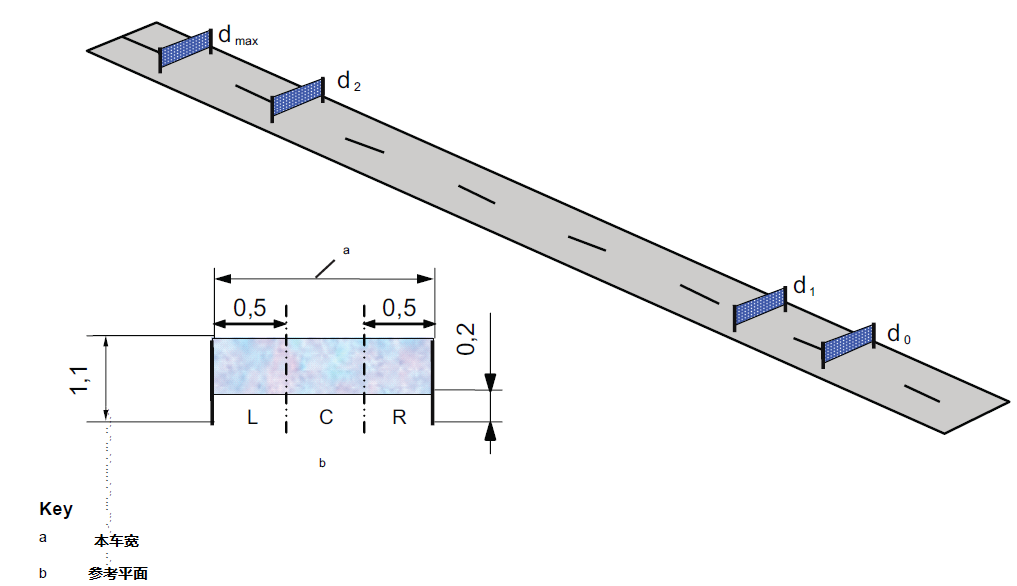
\includegraphics[width=0.7\linewidth]{figures/longdetection}
	\caption{纵向检测范围}
	\label{fig:longdetection}
\end{figure}

\begin{itemize}
	\item 在$d_\text{max}$距离处采用测试目标A;
	\item 在$d_0,d_1,d_2$距离处采用测试目标B;
	\item $d_2$特指前方本车75 m的距离;
	\item 探测距离测试应在动态条件下进行,静态测试也可作为补充选择。
\end{itemize}
最大探测目标车的时间:目标出现后,2s内就能探测到目标。

\sclause{目标识别测试}\label{7.4}
\ssclause{初始条件}
两辆同型号的车辆在本车的前方以$v_\text{vehicle-start}$速度同向行驶,两车纵向中心线间的距离为$\SI{3.5}{m}\pm \SI{0.25}{m}$,车宽在$\SI{1.4}{m}\sim \SI{2}{m}$间。本车在车间时距控制模式下稳定跟随其中一辆前车行驶(该车即为目标车),车间时距为$\tau_\text{max}(v_\text{vehicle-start})$,设定车速大于$v_\text{vehicle-end}$。本车与目标车纵向中心线间的横向偏差小于0.5m(见图~\ref{fig:startconditions})
\[v_\text{vehicle-end} = \SI{27}{m/s}(\sim \SI{100}{km/h})\]
\begin{figure}[htbp]
	\centering
	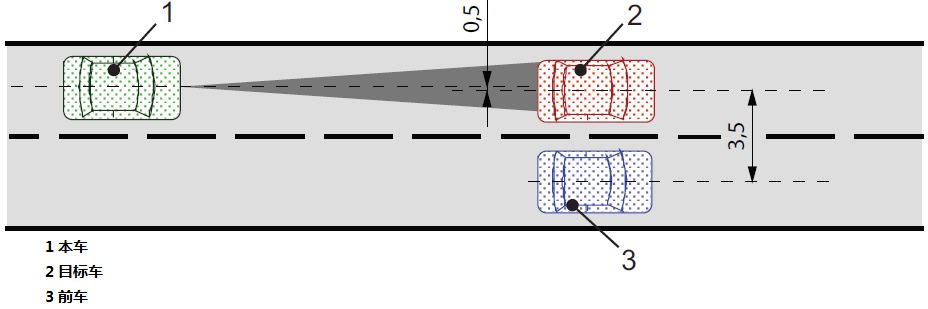
\includegraphics[width=0.7\linewidth]{figures/Startconditions}
	\caption{目标测速-初始条件}
	\label{fig:startconditions}
\end{figure}

\begin{anote}
如果无法达到上述速度,则$v_\text{vehicle-end} = \SI{22}{m/s}(\sim \SI{80}{km/h})$。其中$v_\text{vehicle-start} = v_\text{vehicle-end} -\SI{3}{km/h}$。
\end{anote}
\ssclause{测试过程}
目标车加速至$v_\text{vehicle-end}$,如果本车在FSRA状态下超过相邻车道上的前车,见图~\ref{fig:endcondition},则测试合格。
\begin{figure}[htbp]
	\centering
	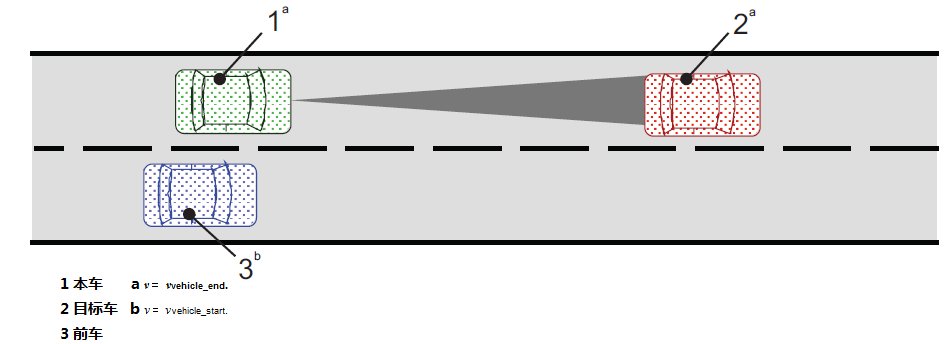
\includegraphics[width=0.7\linewidth]{figures/endtestdis}
	\caption{目标识别-结束条件}
	\label{fig:endcondition}
\end{figure}


\sclause{弯道适应能力测试}
本测试应考虑对道路几何结构参数进行预测,同时兼顾FSRA系统传感器的视野范围。由于道路几何结构参数预测方法和前方车辆探测方法不同,故需要设计一驾驶场景以便进行弯道适应能力测试。
\ssclause{测试场地}\label{7.6.1}
测试场地适用于FSRA的II,III,IV型系统。

测试车道由某一半径的圆或一段足够长的曲线构成,弯道半径的取值范围为(80\%〜100 \%)$R_\text{min}$。测试车道为双向车道,即可沿顺时针和逆时针方向行驶。对车道标线、护栏等设施没有限制要求 (见图~\ref{fig:outlinetrack})。
\begin{figure}[htbp]
	\centering
	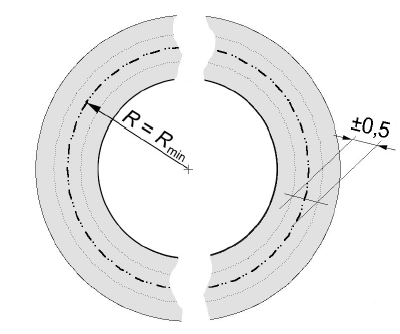
\includegraphics[width=0.4\linewidth]{figures/outlinetrack}
	\caption{弯道车道测试示意}
	\label{fig:outlinetrack}
\end{figure}

\begin{itemize}
	\item 对于II型系统,$R_\text{min,II} = \SI{500}{m}$;
	\item 对于III型系统,$R_\text{min,III} = \SI{250}{m}$;
		\item 对于IV型系统,$R_\text{min,IV} = \SI{125}{m}$。
\end{itemize}
\ssclause{用于弯道适应能力测试的目标车}
在目标车尾部安装如所述的测试目标A,目标车应放置在车辆后端的中部,高度离地面0.6±0.1m。

其余未被遮盖的表面按如下原则进行隐藏处理:使车辆尾部的雷达散射截面RCS不大于(移去测试目标A以后)或使其反射率不大于测试目标的20\%。
\ssclause{驾驶场景}
本车以车间时距控制模式跟随同一车道上的目标车(二者纵向中心线间的横向偏差为±0.5 m)。

 测试之前,本车和目标车应满足\ref{fig:startconditions}给定的初始条件,测试过程的具体细节见表\ref{tab:wandao}和图\ref{fig:trackexample}。
\begin{table}[htbp]
	\centering
	\caption{弯道适应能力测试条件}
	\begin{tabular}{|p{7em}|cc|cc|}
		\hline
		项 目   & \multicolumn{1}{p{10em}|}{测试前准备} & \multicolumn{1}{p{4em}|}{初始条件} & \multicolumn{1}{p{6.25em}|}{第一测试环节} & \multicolumn{1}{p{6em}|}{第二测试环节} \\
		\midrule
		\multicolumn{5}{|p{35.44em}|}{目标车} \\
		\midrule
		速度   & \multicolumn{2}{p{10em}|}{$v_\text{circle-start} =$ 常量} & \multicolumn{1}{p{9em}|}{使车速降低$3.5\pm 0.5\si{m/s}$} & \multicolumn{1}{p{6em}|}{$v_\text{circle}=\text{常数} =v_\text{circle-start} - (3.0\pm 1\si{m/s})$} \\
		\midrule
		时间    & \multicolumn{1}{p{10em}|}{至少10 s} & \multicolumn{1}{p{4em}|}{时间触发0 s} & \multicolumn{1}{p{6.25em}|}{2 s} & \multicolumn{1}{p{4.19em}|}{—} \\
		\midrule
		行驶轨迹的半径 & \multicolumn{1}{p{14.625em}|}{不小于~\ref{7.6.1}中的定义值可能改变} & \multicolumn{3}{p{13.94em}|}{R为常数见~\ref{7.6.1}} \\
		\midrule
		\multicolumn{5}{|p{35.44em}|}{本车} \\
		\midrule
		速度    & \multicolumn{2}{c|}{$\leq\SI{0.5}{m/s^2}$} & \multicolumn{2}{c|}{观测本车减速度} \\
		\midrule
		行驶轨迹半径 & \multicolumn{1}{l|}{不小于~\ref{7.6.1}中的$R$,定义值可能改变} & \multicolumn{3}{c|}{R为常数见~\ref{7.6.1}} \\
		\midrule
		到目标车辆的车间时距 & \multicolumn{2}{c|}{$\tau_\text{max}(v_\text{circle-start})\pm 25\%$} & \multicolumn{2}{c|}{由FSRA控制,观测车间时距} \\
		\bottomrule
	\end{tabular}%
	\label{tab:wandao}%
\end{table}%

\begin{figure}[htbp]
	\centering
	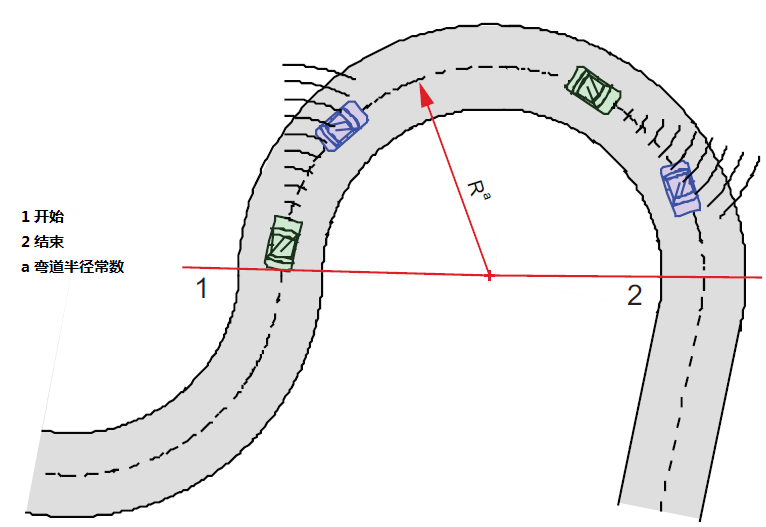
\includegraphics[width=0.4\linewidth]{figures/trackexample}
	\caption{测试轨道布置示意图}
	\label{fig:trackexample}
\end{figure}

开始测试时,目标车的初始速度为:
\[v_\text{circle-start}=\min
[(a_\text{laterl-max}\times R)^{1/2},v_\text{vehicle-max}]\pm \SI{1}{m/s}\]
式中的$a_\text{laterl-max}$取决于弯道半径(见附录):
\begin{itemize}
	\item 当$R=R_\text{min.II} = \SI{500}{m}$时,$ a_\text{lateral-max} = 2.0 m/s^2$;
	\item 当$R=R_\text{min.III} = \SI{250}{m}$时,$ a_\text{lateral-max} = 2.3 m/s^2$;
	\item 当$R=R_\text{min.IV} = \SI{125}{m}$时,$ a_\text{lateral-max} = 2.3 m/s^2$
\end{itemize}

选择适当时机,使目标车减速,观察本车的反应。正常情况下,在车间时距减小至$\frac{2}{3}\tau_\text{max}$之前,本车就会因与目标车车距减小而开始减速。


\infannex{技术参考}
\sclause{激光雷达一测试目标的CTT参数}
\sclause{立体角$\varOmega$}
立体角$\varOmega$为激光照射区域面积与球面半径平方的比值(见图\ref{fig:solidangle})
\[\varOmega = \frac{A}{d^2_A}\times\varOmega_0\]
其中:
\begin{itemize}
	\item $\varOmega$,立体角,单位球面度(sr);
	\item $A$,可用区域面积;
	\item $d_A$,光源与可用区域A之间的距离;
	\item $\varOmega_0$,光源发光范围的交体角
\end{itemize}
\begin{figure}
	\centering
	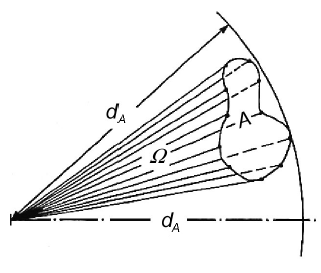
\includegraphics[width=0.4\linewidth]{figures/solidangle}
	\caption{立体角}
	\label{fig:solidangle}
\end{figure}

\sclause{辐射强度$I$}
辐射强度$I$,指光源在单位立体角$\varOmega$内的辐射能量$\Phi$。
\[I_\text{ref} =\frac{d\Phi_\text{ref}}{d\varOmega_1}\]

其中:
\begin{itemize}
	\item $I_\text{ref}$,反射光源在某一特定方向上的辐射强度,在接收器前测量获取T单位为瓦特/球面度 (W/sr);
	\item $\Phi_\text{ref}$,来自反射源的辐射能量,单位为瓦特(W);
	\item $\varOmega_1$,反射光的立体角,单位为球面度(sr)
\end{itemize}
\sclause{照度$E$}
照度指光源辐射能量与受照面积的比值,也即照射密度。
\[E_\text{t} =\frac{d\Phi_\text{t}}{dA}\]

其中,$E_\text{t}$,单位为瓦特每平方米($\si{w/m^2}$)
\sclause{测试目标参数CCT}
测试目标由反射体的参数定义,该参数表示一辆表面较脏并且没有安装向后反射体的轿车的反射率。
\[\text{CCT} =\frac{I_\text{ref}}{E_t}\]

具有CTT参数的反射体(见图\ref{fig:receiver})的反射具有一定的空间分布,其立体角不小于 \num{8e-3}sr。
\begin{figure}
	\centering
	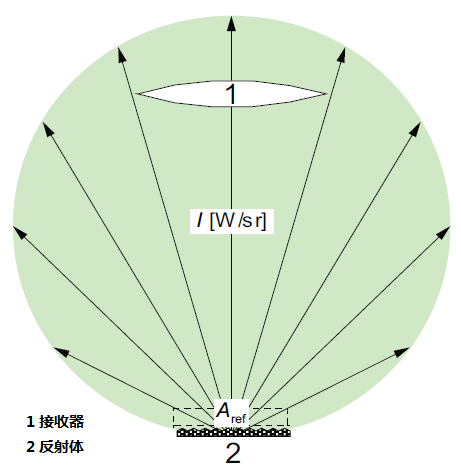
\includegraphics[width=0.5\linewidth]{figures/receiver}
	\caption{接受示意图}
	\label{fig:receiver}
\end{figure}


测试目标的CTT参数仅用于描述反射体对红外的反射能力(衰减特性)作为测试方法,采用锥形反射体(即反射面缩小为一点,见图\ref{fig:transmitter})即可满足要求;当然,只要反射面的反射率不超过设定值,也可采用更大的反射面。
\begin{figure}
	\centering
	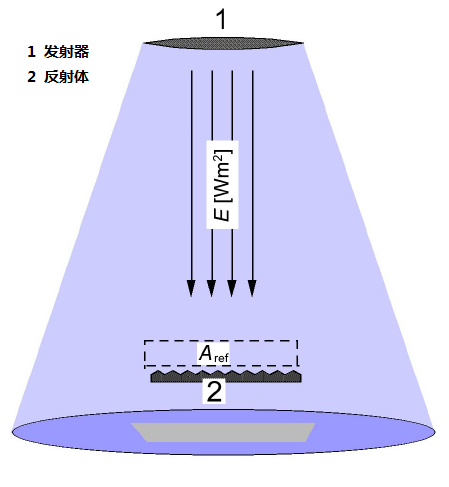
\includegraphics[width=0.5\linewidth]{figures/transmitter}
	\caption{发射示意图}
	\label{fig:transmitter}
\end{figure}
\sclause{反射体尺寸}
应定义反射体(见图\ref{fig:reflector})的尺寸大小经验表明,在与车辆相关的应用中,朗伯反射体尺寸取值在\SI{1.7}{cm^2}左右时的效果最佳。也可采用三层反射的方法,此时反射体尺寸大约为\SI{20}{cm^2}左右。
\begin{figure}[htbp]
	\centering
	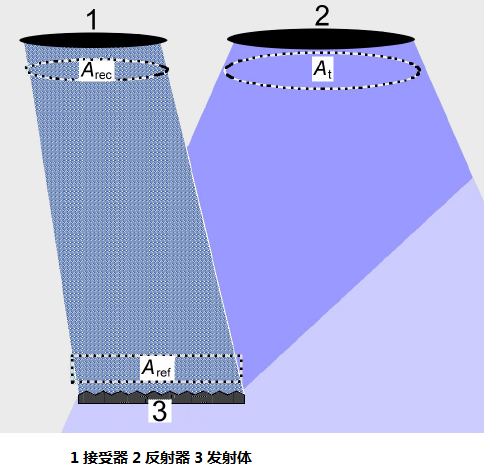
\includegraphics[width=0.5\linewidth]{figures/reflector}
	\caption{发射示意图}
	\label{fig:reflector}
\end{figure}
朗伯反射体可以反射一个球面内(见图~\ref{fig:lambert})的全部能量。
\[\Phi_\oplus = \pi \times I_0\times \varOmega_0\]

其中,
\begin{itemize}
	\item $\Phi_\oplus$,辐射能量,单位为瓦特(W);
	\item $I_0$,辐射强度,单位为瓦特每球面度(W/sr);
	\item $\varOmega_0$,立体角,单位为球面度(sr)
\end{itemize}
\begin{figure}[htbp]
	\centering
	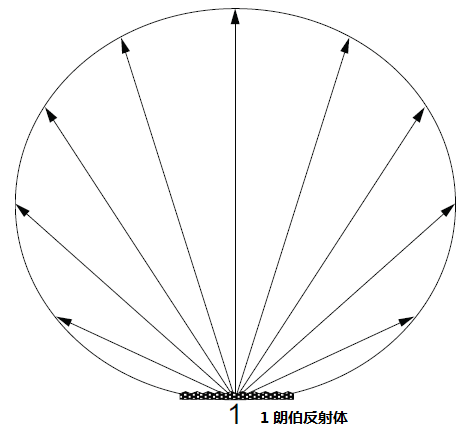
\includegraphics[width=0.4\linewidth]{figures/lambert}
	\caption{朗伯反射体}
	\label{fig:lambert}
\end{figure}
\sclause{锥体型测试目标的雷达信号散射截面定义}
\begin{itemize}
	\item 测试目标的雷达信号散射截面定义为RCS=(10±3)\si{m^2}。对于目前常用的频率(如60 GHz、 77 GHz、90 GHz),10 \si{m^2}的范围至少可以覆盖公路上95\%的车辆 。
	\item 测试目标的外观见图~\ref{fig:cubereflector}。
	\item 雷达散射截面(RCS)计算公式:
	\[\text{RCS} = \frac{4\times\pi\times L^4}{3\times \lambda^2}\]
	其中,
	
	$\lambda$,波长
	
	$L$,雷达反射体一面的长度。
\end{itemize}
\begin{figure}[htbp]
	\centering
	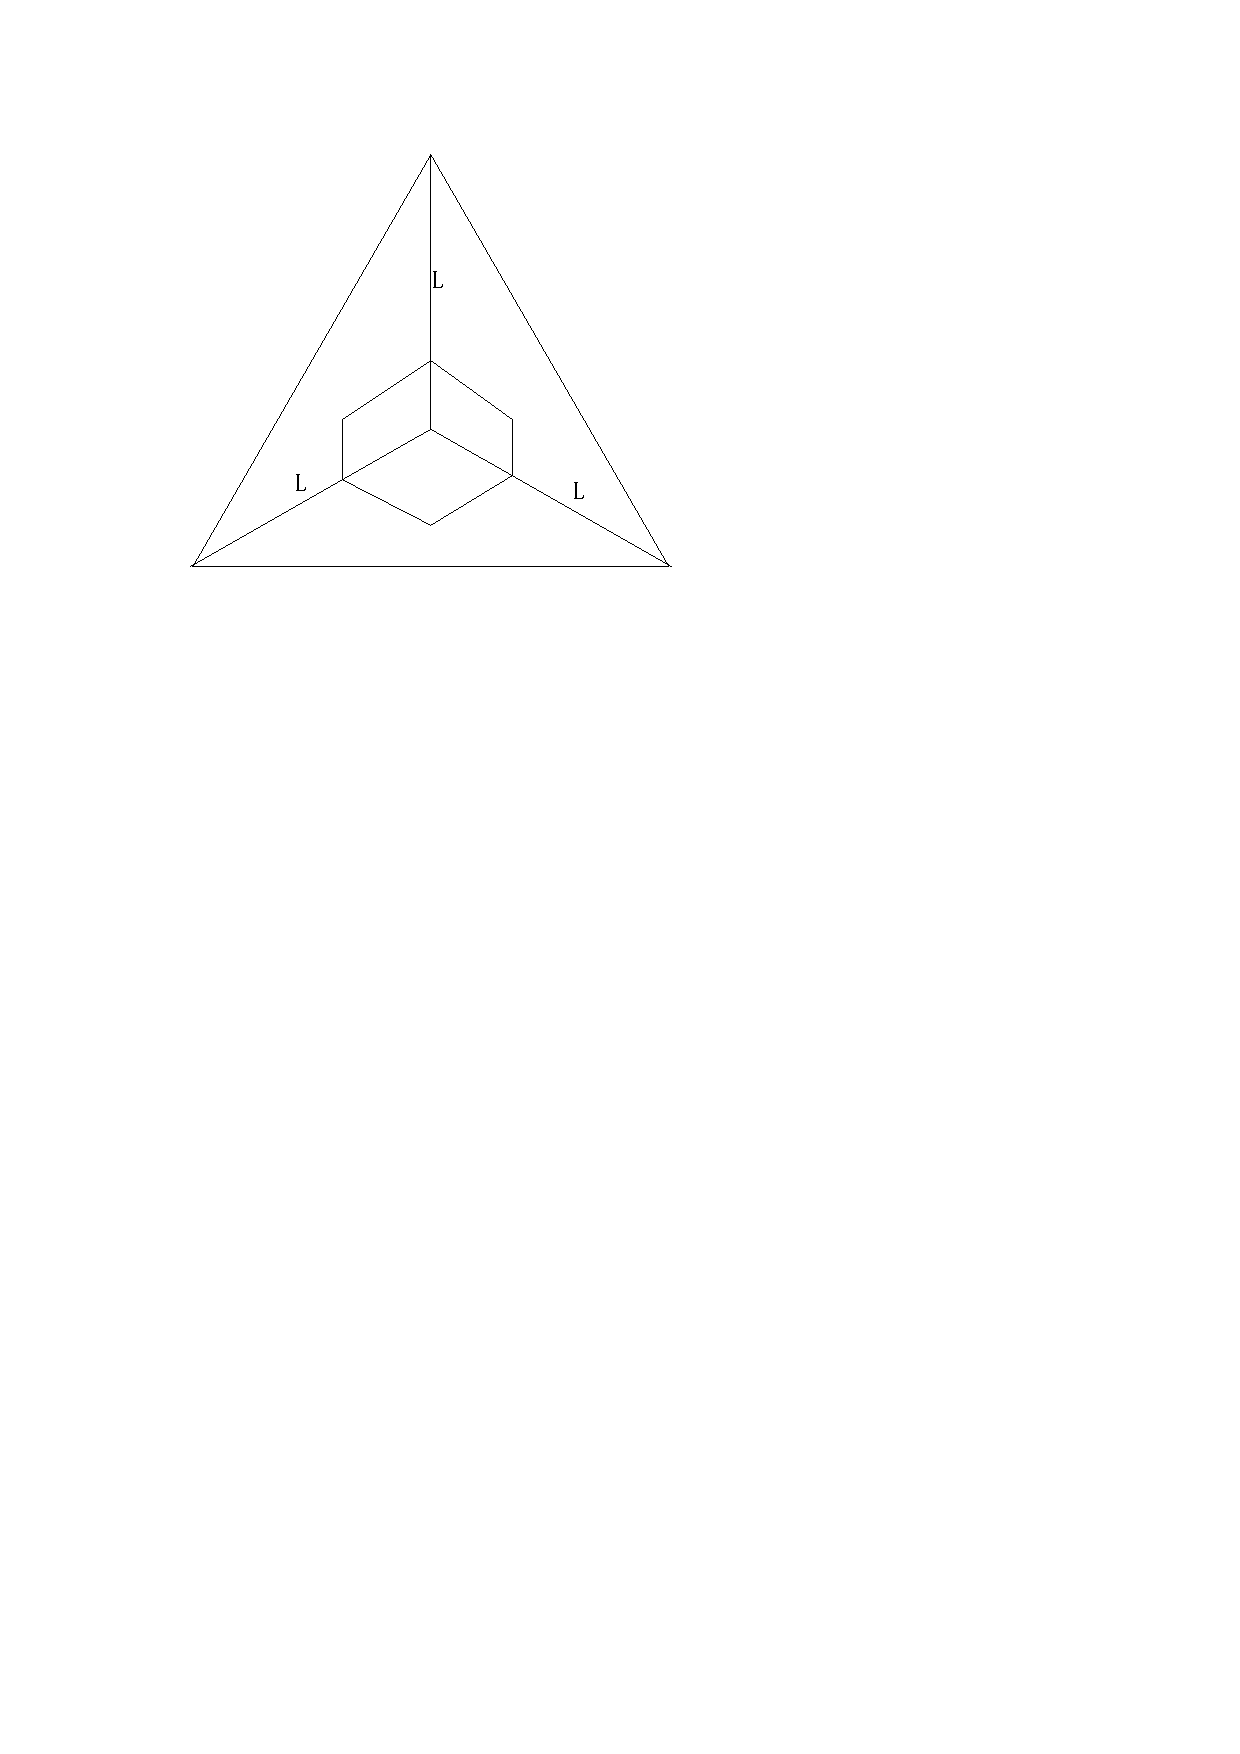
\includegraphics[width=0.4\linewidth]{figures/cubereflector}
	\caption{立方反射体}
	\label{fig:cubereflector}
\end{figure}
\bibannex
\begin{references}
	\reference{ISO 15622,}{Transport information and control systems — Adaptive Cruise Control Systems —
		Performance requirements and test procedure.}{}
	\reference{IEC 60825-1,}{Safety of laser products — Part 1: Equipment classification and requirements.}{}
	\reference{United Nations Economic Commission for Europe, Regulation No. 13-H (ECE-R 13-H),}{Uniform
		provisions concerning the approval of passenger cars with regard to braking}{}\label{ref:UN}
\end{references}
\end{document}